\section{Zeeman-Effekt}\label{sec:zeeman}
Der Zeeman-Effekt beschreibt die Aufspaltung der Energieniveaus einzelner Zustände 
in einem Magnetfeld. Spin und Bahndrehimpuls bewirken ein magnetisches Moment, auf welches 
ein äußere Magnetfeld wirken kann. Quantenmechanisch kann dies durch den Hamiltonoperator 
beschrieben werden, der die Interaktion mit einem äußeren Feld beschreibt \cite{Sakurai}:
\begin{equation}
    \hat H_\mathrm{int} = -\frac{q}{2m_\mathrm e}\qty(\hat{\vec L} + 2\hat{\vec S})\cdot \vec B.
    \label{eq:zeeman_hamilton}
\end{equation}

In diesem Versuch wird die Aufspaltung an Cadmium beobachtet. Das äußere Elektron sieht 
aufgrund der Wahrscheinlichkeitsverteilung in erster Näherung den Kern mit den inneren 
Schalen effektiv als nur ein Teilchen, womit die Berechnung der Energieniveaus 
äquivalent zum Wasserstoffatom betrachtet werden kann. Da dieses durch eine gerade 
Elektronenzahl keinen Gesamtspin 
besitzt und das Magnetfeld homogen ist, vereinfacht sich \cref{eq:zeeman_hamilton} zu 
\begin{equation*}
    \hat H_\mathrm{int} = \frac{eB}{2m_\mathrm e}\hat{L_z},
\end{equation*}
wobei die Elektronenladung eingesetzt wurde und das Magnetfeld per Konvention in die z-Achse zeigt.
Da bei kugelsymmetrischem Potenzial die z-Komponente des Drehimpulsoperators mit dem restlichen Hamiltonoperator
des Atoms kommutiert, ergibt sich eine Verschiebung des Energieniveaus von
\begin{equation*}
    \Delta E = \frac{e\hbar}{2m_\mathrm e}m_jB \equiv \mu_\mathrm B m_j B
    \label{eq:energy_zeeman}
\end{equation*}

mit dem Bohrschen Magneton \cite{Demtröder:829119}
\begin{equation}
    \mu_B = \SI{9.274015}{\joule\per\tesla}.
    \label{eq:magneton}
\end{equation}
Weil hier elektrische Dipolübergänge betrachtet werden, gilt die Auswahlregel 
$\Delta m = \{\pm 1, 0\}$ \cite{Demtröder:829119}, wobei einer Differenz 
von null linear polarisiertes Licht (im folgenden als $\pi$ bezeichnet) und einer Differenz von $\pm 1$
zirkular polarisiertes Licht ($\sigma^+$ für links zirkular und $\sigma^-$ für rechts zirkular) 
zugeordnet werden kann.
Für $\pi$-Polarisation kann daher keine Energieverschiebung beobachtet werden, für 
$\sigma^\pm$-Polarisation eine Verschiebung von 
\begin{equation}
    \delta E = \pm \mu_\mathrm B B
    \label{eq:normal_zeeman}.
\end{equation}
Unabhängig von der Drehimpulsquantenzahl kann somit beim hier beschriebenen 
normalen Zeeman-Effekt immer nur eine Aufspaltung in drei Linien beobachtet werden,
weshalb die Entartung nur teilweise aufgehoben werden kann.

In \cref{fig:zeeman_übergänge} ist das Übergangsschema für die Übergänge ${}^1D_2\rightarrow {}^1P_1$
des Cadmiumatoms dargestellt. Die Wellenlänge des Übergangs ist $\lambda_0 = \SI{644}{\nano\meter}$
und entspricht rotem Licht. Dieser Übergang wird in diesem Versuch untersucht.

\begin{figure}
    \centering
    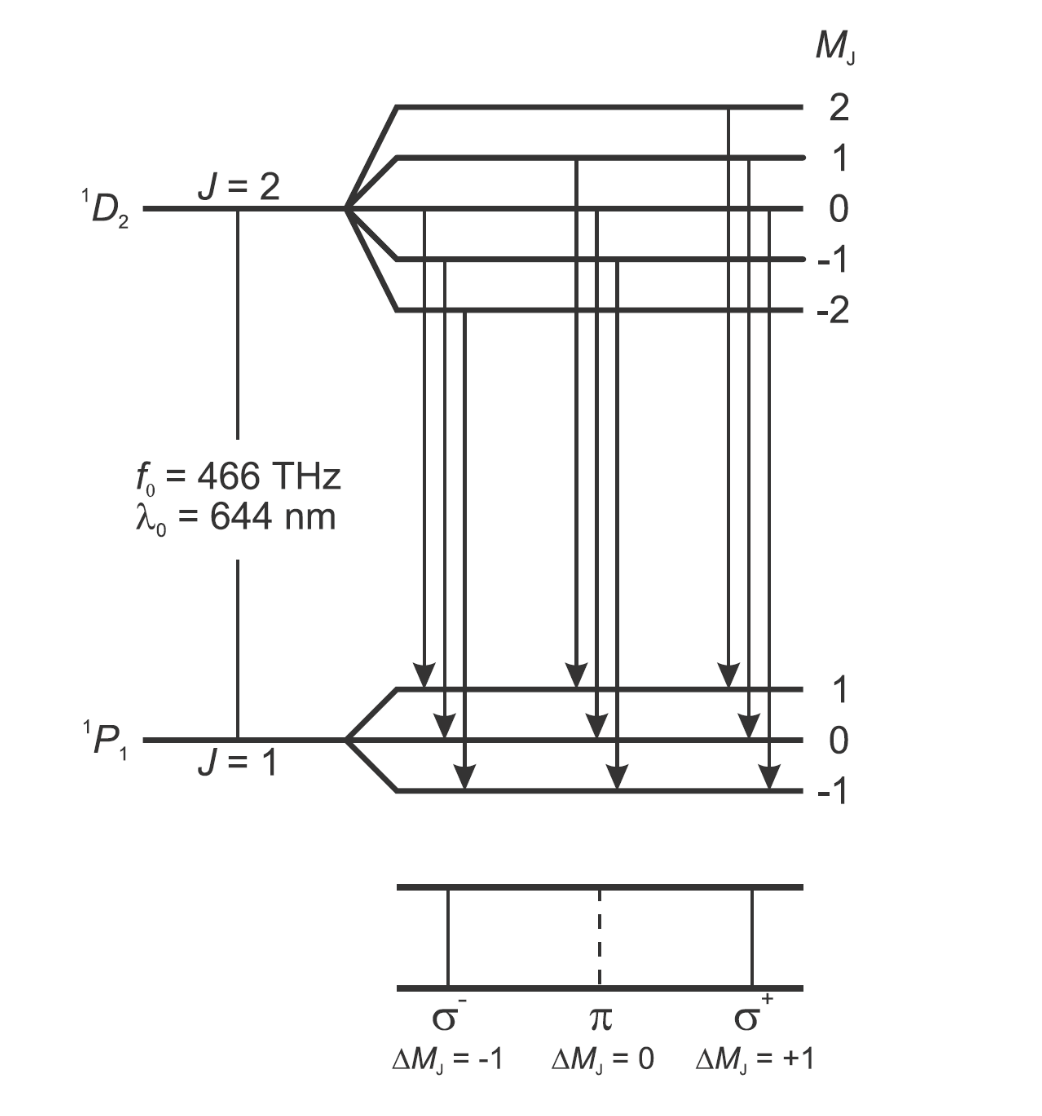
\includegraphics[width=0.6\linewidth]{../figs/zeeman_übergänge}
    \caption{Übergangsschema von Cadmium für die Singulett-Zustände ${}^1D_2\rightarrow {}^1P_1$. 
        Zusehen sind jeweils drei Übergangsgruppen mit je drei Übergängen, die untereinander
        entartet sind, die Entartung zwischen einander jedoch durch den Zeeman-Effekt aufgehoben wird. Darunter 
        ist die durch die Auswahlregeln bestimmte Polarisation des abgestrahlten Lichts aufgetragen. 
        \cite{zeeman_handblatt}}
    \label{fig:zeeman_übergänge}
\end{figure}

\subsection{Versuchsaufbau}
Der Aufbau zur Untersuchung des Zeeman-Effekts ist in \cref{fig:zeeman_aufbau} skizziert. Eine 
Cadmiumlampe wird zwischen ein Magnetfeld festgehalten, welches durch zwei in Reihe 
geschalteten stromdurchflossenen Spulen erzeugt wird. Die Spulen können 
um die vertikale Achse gedreht werden, um die Richtung 
des Magnetfeldes in Bezug zur Beobachtungsrichtung verändern zu können. 
Das Licht der Lampe wird mit einer Kondensorlinse 
$f=\SI{150}{\mm}$ kollimiert mit leichter Konvergenz, um nachher am Etalon verschieden Einfallswinkel zu 
erzeugen. 

Das eingebaute Fabry-P\'erot-Etalon ist eine planparallele Glasschicht, welche 
beidseitig mit teildurchlässigen Spiegeln beschichtet ist. Durch ständige Reflexion innerhalb der Glasschicht
wird ein Strahlenbündel erzeugt, welches durch Gangunterschiede untereinander interferiert. 
Das hier benutzte Etalon hat einen Brechungsindex von $n=1.457$ und einem Reflexionsgrad $R=0.85$.
Mit einer weiteren Sammellinse $f=\SI{150}{\mm}$ wird das Licht am Okular scharf abgebildet, an 
dem durch die entstandene Interferenz konzentrische Ringe Beobachter sein können. Davor wird mit einem 
Interferenzfilter das rote Licht bei $\SI{644}{\nm}$ gefiltert.

\begin{figure}[h]
    \centering
    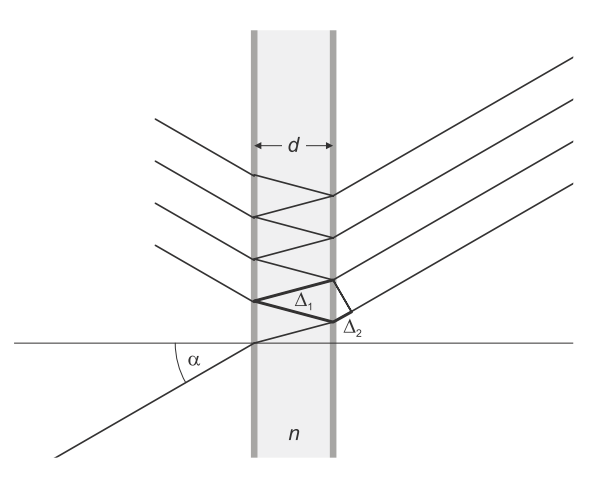
\includegraphics[width=0.6\linewidth]{../figs/etalon}
    \caption{Funktionsweise eines Fabry-P\'erot-Etalon. $\alpha$ bezeichnet den Einfallswinkel 
        eines Lichtstrahls in den Etalon mit Dicke $d$ bei Brechungsindex $n$.
        $\Delta_1$ und $\Delta_2$ bezeichnen die Gangunterschiede, die zur Interferenz zweier 
        transmittierter Strahlen führen.
        \cite{zeeman_handblatt}}
    \label{fig:etalon}
\end{figure}

\begin{figure}[h]
    \centering
    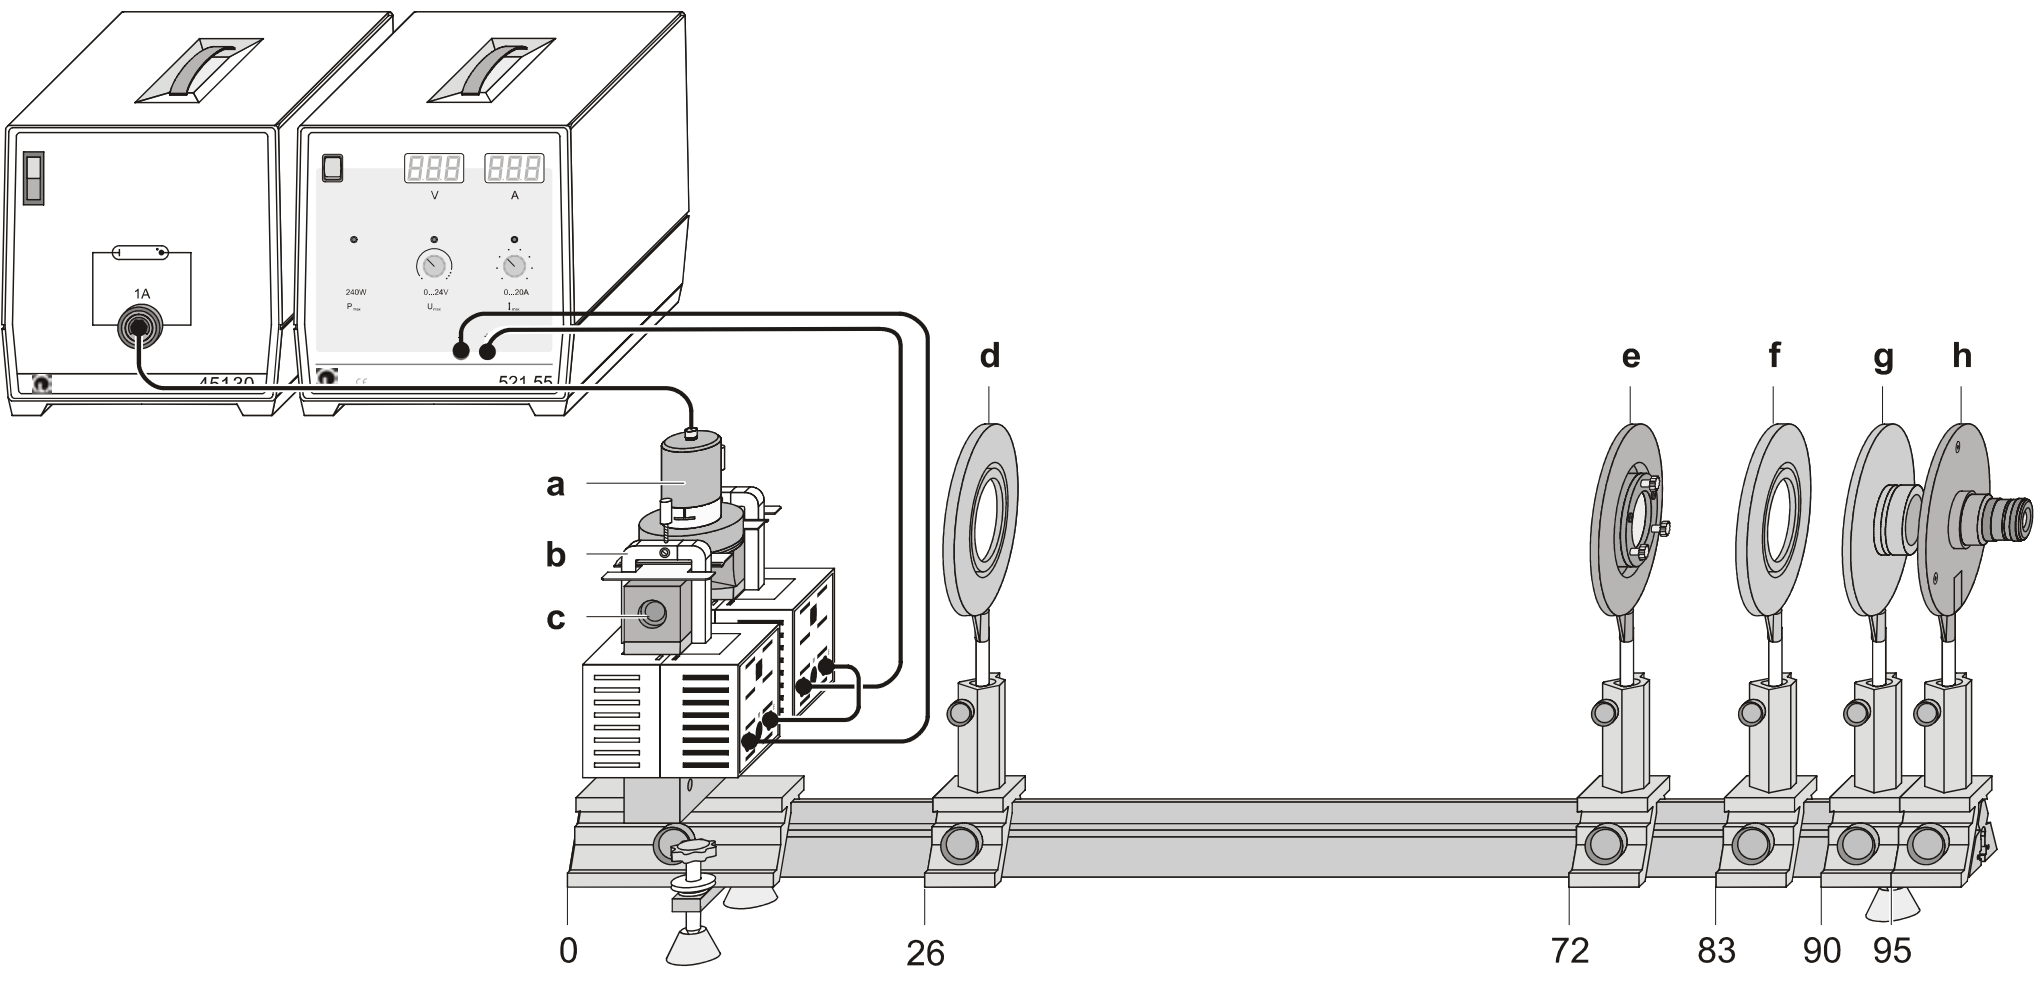
\includegraphics[width=0.7\linewidth]{../figs/zeeman_aufbau}
    \caption{Aufbau zur Messung des Zeeman-Effekts. \abf a zeigt die Cadmiumlampe mit Klammern
        \abf b und Polschuhe \abf c. \abf d zeigt die Kondensorlinse, \abf e das Etalon, \abf f 
        die Abbildungslinse, \abf g das Interferenzfilter und \abf h das Okular mit Strichskala. 
        \cite{zeeman_handblatt}}
    \label{fig:zeeman_aufbau}
\end{figure}

\subsection{Untersuchung der Transversal- und Longitudinalkonfiguration}
Durch das Drehen der Spulen lässt sich die Polarisation der emittierten Strahlung 
untersuchen. Hierbei werden zwei Konfigurationsmöglichkeiten gesondert betrachtet.
Klassisch lässt sich die Polarisations- und Strahlrichtung der Übergangsstrahlung 
mit dem Lorentz-Modell beschreiben, wo eine Schwingungsgleichung mit der Lorentzkraft als 
treibende Kraft angesehen wird. Dabei sind $\pi$- und $\sigma^\pm$-Strahlung die Eigenmodi 
der Lösung. Diese sind in \cref{fig:zeeman_polarisation} skizziert. Zu sehen ist hierbei, 
dass sich jede Lösung als schwingender Dipol interpretieren lässt, wobei für $\sigma^\pm$ 
zwei senkrecht zueinander stehenden Dipole mit einer $\SI{90}{\degree}$-Phasenbeziehung 
betrachtet werden.

Da Dipole nicht in Bewegungsrichtung abstrahlen, kann in longitudinaler 
Beobachtungsrichtung (parallel zum Magnetfeld) nur die zirkular polarisierte $\sigma^\pm$-Strahlung
beobachtet werden. Bei transversaler Konfiguration sind alle drei Modi sichtbar mit dem 
Unterschied, dass $\sigma^\pm$ hier linear polarisiert ist und räumlich um $\SI{90}{\degree}$
zur $\pi$-Polarisation gedreht.

\subsubsection{Transversalkonfiguration}
In Transversalrichtung können $\sigma^\pm$- sowie $\pi$-Strahlung beobachtet werden, wobei 
diese Modi linear polarisiert sind und senkrecht zueinander stehen. Mit einem Polarisationsfilter 
lässt sich somit $\pi$ und $\sigma$ voneinander trennen, $\sigma^+$ und $\sigma^-$ sind jedoch nicht 
unterscheidbar voneinander. Vor das Etalon wird der Polarisationsfilter befestigt und 
beim Einschalten des Magnetfeldes das Bild beobachtet. Die optische Achse 
des Filters steht auf $\SI{0}{\degree}$, wenn Diese senkrecht zur optischen Bank
steht. Erwartet wird das Verschwinden der inneren Ringe bei einer Filterausrichtung von 
\SI{0}{\degree}, da in diesem Falle die optische Achse des Filters senkrecht zum B-Feld und damit 
zur Polarisationsachse des $\pi$-Lichts steht. Damit ist das Verschwinden der äußeren Ringe 
bei \SI{90}{\degree} zu erwarten.

In \cref{fig:transversal_konfiguration} sind die Interferenzringe abgebildet. Durch das Anlegen
eines Magnetfeldes wurde die Aufspaltung der Ringe in einen hellen mittleren 
Ring und zwei leicht dunklere daneben deutlich. Aufgrund des Auflösungsvermögens und möglicherweise 
einer Überbelichtung konnten die Details des Bildes auf der Aufnahme nicht kenntlich
gemacht werden. Bei einer Polarisationsfiltereinstellung von \SI{0}{\degree} verschwinden
die inneren Ringen, bei \SI{90}{\degree} die Äußeren. Dies entspricht dem erwarteten Verhalten, 
weshalb daraus geschlossen werden kann, dass das Licht der äußeren Ringe senkrecht zum 
B-Feld polarisiert ist und das Licht der inneren Ringe parallel dazu.

\begin{figure}[h]
    \centering
    \begin{subfigure}{0.45\linewidth}
        \centering
        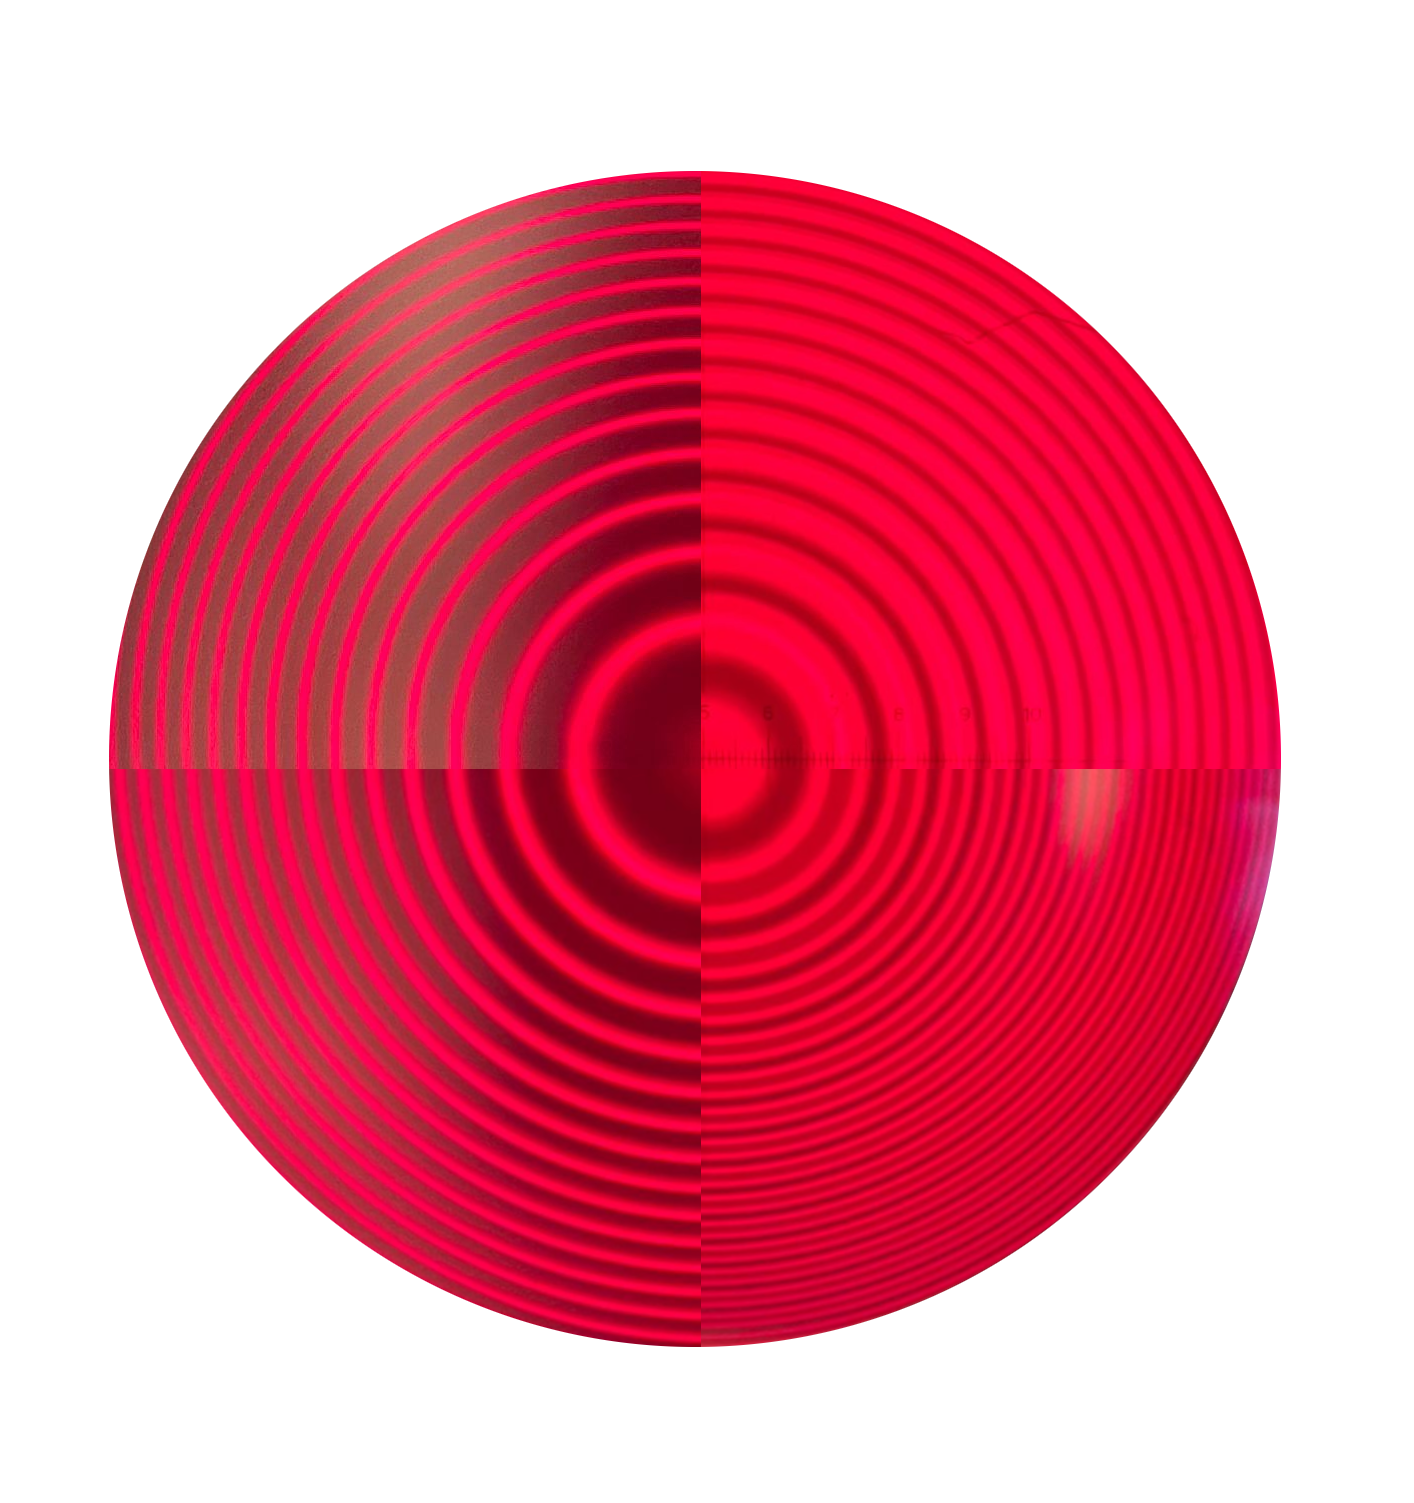
\includegraphics[width=\linewidth]{../figs/transversal_konfig}
        \caption{Transversal Konfiguration: links oben ohne B-Feld, rechts oben mit B-Feld,
            rechts unten mit Filter auf $\SI{0}{\degree}$, links unten mit Filter auf $\SI{90}{\degree}$.}
        \label{fig:transversal_konfiguration}
    \end{subfigure}
    \hspace{.5cm}
    \begin{subfigure}{0.45\linewidth}
        \centering
        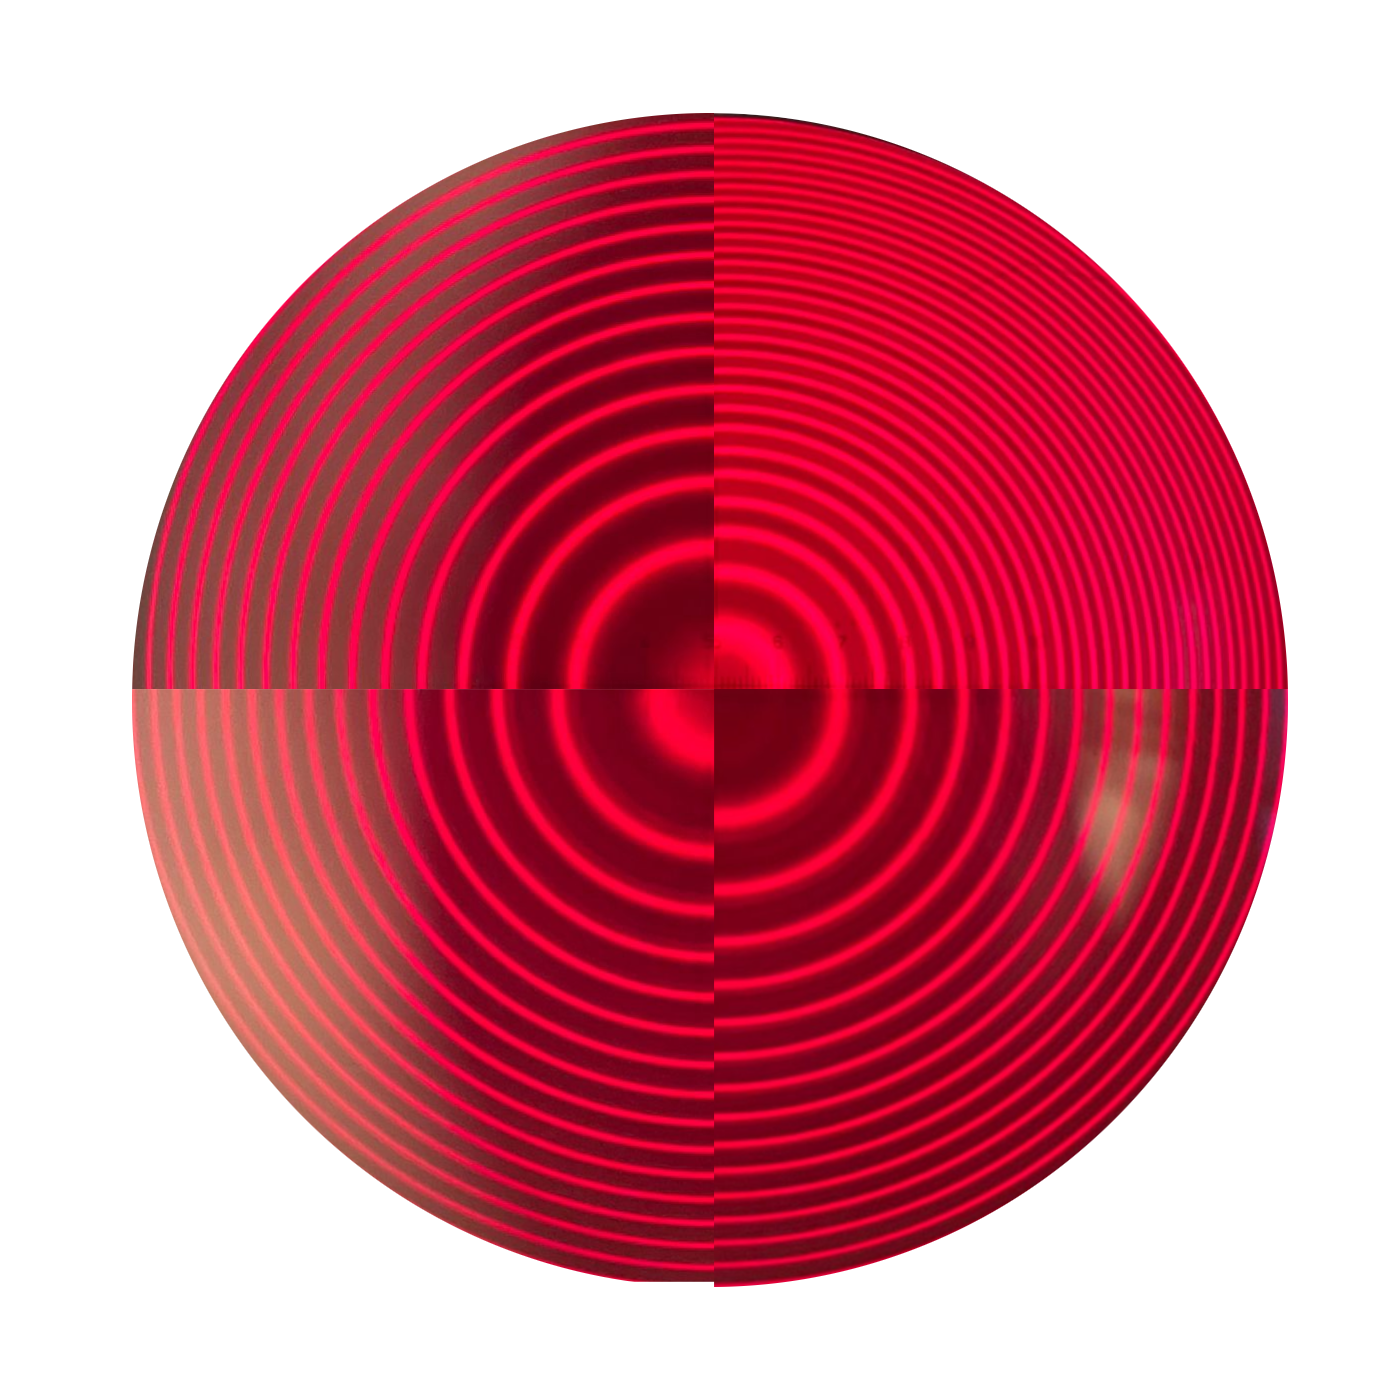
\includegraphics[width=\linewidth]{../figs/longitudinal_konfig}
        \caption{Longitudinal Konfiguration: links oben ohne B-Feld, rechts oben mit B-Feld, 
        rechts unten mit Filter auf $\SI{+45}{\degree}$, links unten mit Filter auf $\SI{-45}{\degree}$. }
        \label{fig:longitudinal_konfiguration}
    \end{subfigure}
    \caption{Aufnahmen der Etalon Interferenzringe bei unterschiedlichen Aufbauten.}
\end{figure}


\subsubsection{Longitudinalkonfiguration}
In longitudinaler Ausrichtung kann nur das $\sigma^\pm$-Licht beobachtet werden. Um zu zeigen, 
dass beide Wellen zirkular und entgegengesetzt polarisiert sind, wird vor dem Polarisationsfilter 
eine $\lambda/4$-Wellenplatte befestigt, welche die Phase des elektrischen Feldes parallel 
zur optischen Achse um eine viertel Wellenlänge verschiebt und somit zirkulares Licht 
linear polarisieren kann. Per Definition entsprechen $\sigma^\pm$ die komplexen Vektoren des 
elektrischen Feldes 
$\vb E_\mathrm{\sigma^\mp} \propto \vb e_x \mp i\vb e_y$. Ohne Beschränkung der Allgemeinheit wird die optische Achse 
der Wellenplatte auf die y-Achse gesetzt. Bei einer Verzögerung wird die y-Komponente 
um den Faktor $\e^{\pm i\pi /2} = \pm i$ verschoben, womit sich eine Polarisation von 
$\vb E_\mathrm{\sigma^\mp}\propto \vb e_x \pm \vb e_y$ ergibt. Somit ist $\sigma^-$ 
bei einer Ausrichtung des Filters bei \SI{45}{\degree} sichtbar, während $\sigma^+$ Licht 
bei \SI{-45}{\degree} sichtbar wird. 

In \cref{fig:longitudinal_konfiguration} ist die Longitudinalkonfiguration gezeigt. Es ist zu erkennen,
das sich diesmal beim Anlegen eines Magnetfeldes die Linie in nur zwei symmetrisch verteilte Linien 
aufspaltet. Nach Durchgang einer Verzögerungsplatte und einer Filtereinstellung von $\pm\SI{45}{\degree}$
verschwindet wie erwartet jeweils einer der zwei Ringe. Aufgrund der oberen Überlegung 
lässt sich damit der innere Ring $\sigma^-$-Licht zuweisen und $\sigma^+$-Licht dem äußeren Ring.
Auf die Relation, dass $\sigma^-$ kleinere Winkel und $\sigma^+$ größere Winkel zuzuordnen sind, wird 
bei der Bestimmung des Bohr Magnetons weiter eingegangen.


\begin{figure}[htb]
    \centering
    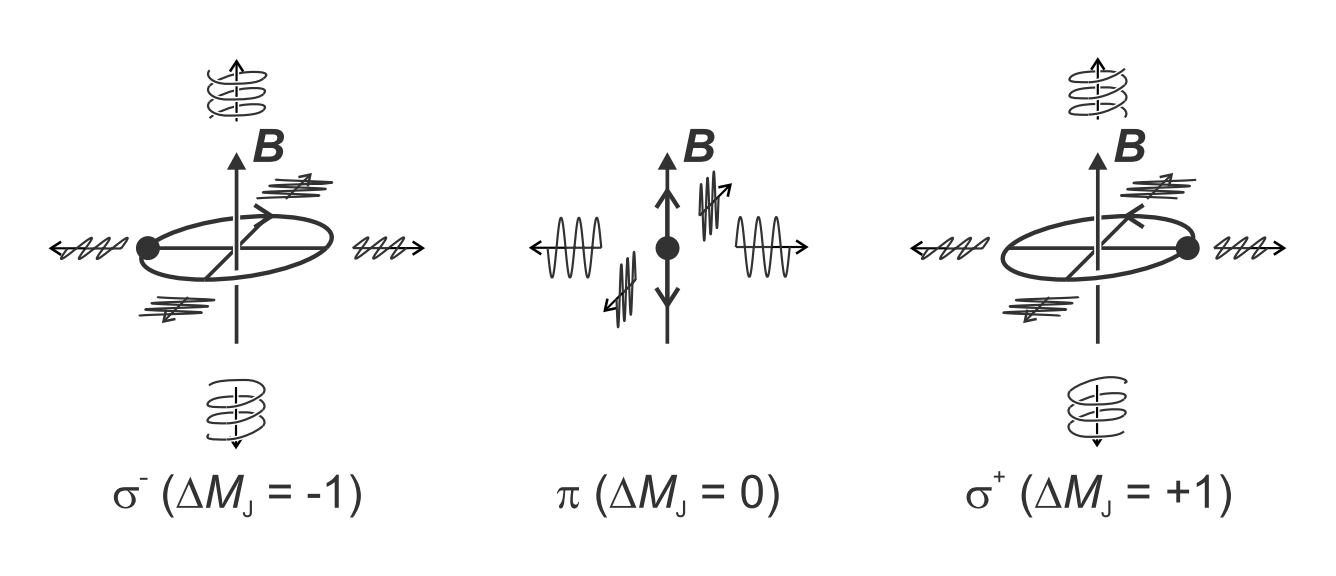
\includegraphics[width=0.6\linewidth]{../figs/zeeman_polarisation}
    \caption{Polarisation der verschiedenen Übergänge. $\pi$-Strahlung ist nur in transversaler 
    Richtung beobachtbar, $\sigma^\pm$-Strahlung in transversaler und in longitudinaler 
    Richtung. \cite{zeeman_handblatt}}
    \label{fig:zeeman_polarisation}
\end{figure}

\subsection{Bestimmung des Bohrschen Magnetons}
Zur Bestimmung des Bohrschen Magnetons wird die Aufspaltung der Linien 
in Transversalkonfiguration mit einer CCD-Kamera gemessen. Diese Messung wird 
bei unterschiedlichen Spulenströmen 40-mal durchgeführt und der Mittelwert 
gespeichert für genauere Ergebnisse. Mit einer Hall-Sonde wird 
zur Kalibration das Magnetfeld in Abhängigkeit des Stroms vor und nach der Durchführung
einer Messung vorgenommen. Durch das Erhitzen der Spulen wird erwartet, dass sich 
die Kalibrationskurve mit der Zeit ändert. Durch zwei Messungen kann damit der Fehler des 
Magnetfeldes bestimmt werden.

Untersucht wird hierbei ein einzelnes Interferenzmaximum nahe des Ringzentrums. Dieses wird 
beim Anlegen eines Magnetfeldes in drei Maxima aufgespalten. An die gemessenen Kurven 
werden drei Gauss-Kurven mit einem linearen Offset angepasst. Die Anpassfunktion kann somit beschrieben werden 
mit 
\begin{equation*}
    f(x, \vec x, \vec \sigma, \vec A, m, n) = \sum_{i=1}^3 \frac{A_i}{\sqrt{2\pi}\sigma_i}
        \exp\qty(-\frac{(x-x_i)^2}{2\sigma_i^2}) +mx + n.
\end{equation*}

Das Programm zur Messung der Einstrahlintensitäten gibt keine dazugehörigen Unsicherheiten an.
Aus diesem Grund müssen diese rekonstruiert werden. Die CCD-Kamera misst Photonen, wodurch 
die Messung pro Pixel als Poisson-verteilt angesehen werden kann mit dazugehörigem Poisson-Fehler \\
$\Delta N = \sqrt{N}$. Die Umrechnung der Zählereignisse in eine Intensität (in Prozent) ist unbekannt, 
weshalb der Fehler mit einem unbekannten Faktor skaliert wird. Für die Anpassungskurve 
ist dieser jedoch irrelevant, da nur der relative Fehler der einzelnen Messpunkte von Bedeutung ist. 
Der Skalierungsfaktor ist daher nicht nötig. Da jedoch nur die relativen Fehler bekannt sind, verliert 
die Berechnung einer Anpassungsgüte, wie dem reduzierten Chi-Quadrat \cite{wiki:reduced_chi_square},
seine Bedeutung, weshalb eine quantitative Bewertung der Anpassungen nicht durchgeführt werden kann.

\begin{figure}
    \centering
    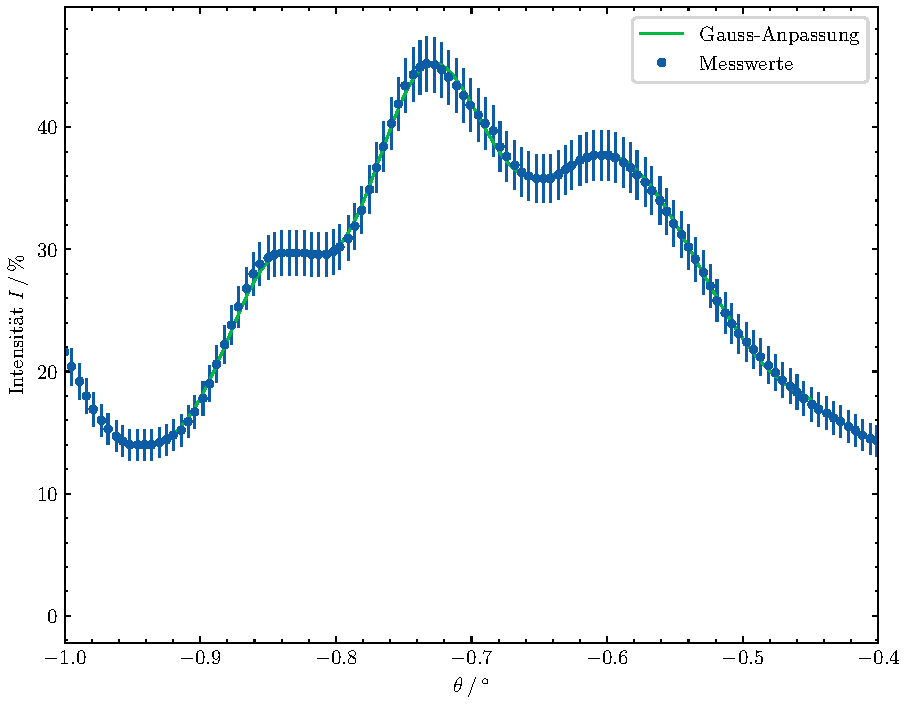
\includegraphics[width=.6\linewidth]{../figs/gauss_i7.9.pdf}
    \caption{Aufspaltung der Maxima bei einem Strom von \SI{7.9}{\ampere}.}
    \label{fig:gauss_i79}
\end{figure}

Eine Anpassungskurve ist beispielhaft in \cref{fig:gauss_i79} gezeigt. Visuell
kann die Anpassung als äußerst erfolgreich angesehen werden. Weitere Diagramme 
sind im \cref{sec:anhang} zu finden.